\newcommand{\convex}{
  \coordinate (p1) at (2,0);
  \coordinate (p2) at (0,2);
  \coordinate (p3) at (1,3.5);
  \coordinate (p3) at (2,4);
  \coordinate (p4) at (4,3.25);
  \coordinate (p5) at (4.5,2);
  \coordinate (p6) at (3.75,1);
  \coordinate (p7) at (2,0);

  \draw (p1) -- (p2) -- (p3) -- (p4) -- (p5) -- (p6) -- (p7);

  \node [anchor=center,circle,draw,fill,inner sep=0.5pt,label={[anchor=south]below:$p_1$}] at (p1) {};
  \node [anchor=center,circle,draw,fill,inner sep=0.5pt,label={[anchor=west]left:$p_2$}] at (p2) {};
  \node [anchor=center,circle,draw,fill,inner sep=0.5pt,label={[anchor=west]above:$p_3$}] at (p3) {};
  \node [anchor=center,circle,draw,fill,inner sep=0.5pt,label={[anchor=west]right:$p_4$}] at (p4) {};
  \node [anchor=center,circle,draw,fill,inner sep=0.5pt,label={[anchor=west]right:$p_5$}] at (p5) {};
  \node [anchor=center,circle,draw,fill,inner sep=0.5pt,label={[anchor=west]below:$p_6$}] at (p6) {};
}

\chapter{Lokalizacja punktu}
% W sytuacji gdy płaszczyznę dzielimy na dwa obszary, z których jeden
% jest nieograniczony, drugi natomiast to wielokąt $P$ (na skutek
% podziału płaszczyzny na dwie części oraz na podstawie twierdzenia
% Jordana o krzywej dla wielokątów wiemy, że $P$ jest prosty) możemy
% przedstawić definicję problemu:

Problem lokalizacji punktu sformułowany jest następująco:

\begin{problem}[Lokalizacja punktu]
  Jeśli dany jest wielokąt prosty $P$ i punkt $z$, sprawdzić czy punkt $z$
  należy do wnętrza $P$.
\end{problem}

Problem ten można rozwiązać w czasie $O(n)$ bez przetwarzania
wstępnego. Przypuśćmy, że istnieje prosta pozioma $l$ przechodząca
przez punkt $z$. Musimy rozważyć kilka przypadków:

\begin{itemize}
\item Jeśli $l$ nie przecina $P$ to $z$ leży na zewnątrz wielokąta.
  \begin{figure}[htp]
    \centering
    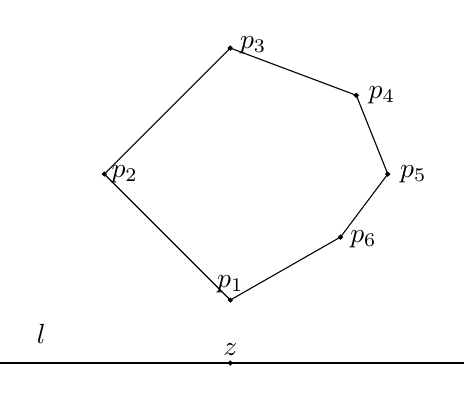
\begin{tikzpicture}[scale=0.8]
      \convex

      \coordinate (z1) at (2,-1);
      \coordinate (l1) at (-1,-1);

      \draw [shorten >=-3cm, shorten <=-1cm] (l1) -- (z1);

      \node [anchor=center,circle,draw,fill,inner
      sep=0.5pt,label={[anchor=south]below:$z$}] at (z1) {};
      \node [label={[anchor=south]above:$l$}] at (l1) {};
    \end{tikzpicture}
    \caption{}
  \end{figure}

\item W przypadku gdy prosta $l$ przecina $P$ i nie przechodzi przez
  żaden z wierzchołków $P$, oznaczamy jako $p_l$ liczbę przecięć $l$ z
  wielokątem $P$. Wiemy, że lewy koniec $l$ leży na zawnątrz $P$, więc
  przesuwając się po prostej $l$ w prawo w kierunku $z$ i przecinając
  brzeg wielokąta i przechodzimy do jego wnętrza. Przy następnym
  przecięciu z brzegiem $P$ znowu znajdziemy się na zewnątrz
  itd. Widzimy stąd, że $z$ jest na zewnątrz wielokąta $P$ dokładnie
  wtedy gdy $p_l$ jest parzyste.

  \begin{figure}[htp]
    \centering
    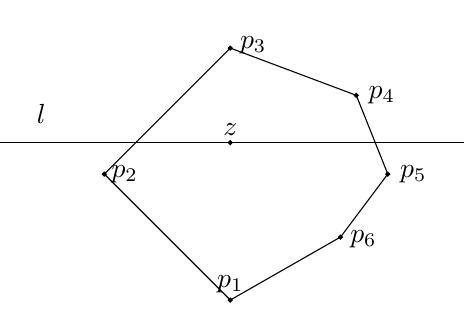
\begin{tikzpicture}[scale=0.8]
      \convex

      \coordinate (z2) at (2,2.5);
      \coordinate (l2) at (-1,2.5);

      \draw [shorten >=-3cm, shorten <=-1cm] (l2) -- (z2);

      \node [anchor=center,circle,draw,fill,inner
      sep=0.5pt,label={[anchor=south]below:$z$}] at (z2) {};
      \node [label={[anchor=south]above:$l$}] at (l2) {};
    \end{tikzpicture}
    \caption{}
  \end{figure}

\item Specjalnym przypadkiem jest ten w którym $l$ przechodzi przez
  jeden lub dwa wierzchołki. W algorytmie rozważamy przecięcia $l$ z
  krawędziami $P$, więc musimy się zabezpieczyć przed sytuacją w,
  której policzylibyśmy przecięcie brzegu $P$ dwukrotnie. Stosujemy tu
  zasadę, że $p_l$ nie zostanie zwiększone dla krawędzi, której jeden
  z wierzchołków znajduję się powyżej prostej $l$.

  \begin{figure}[htp]
    \centering
    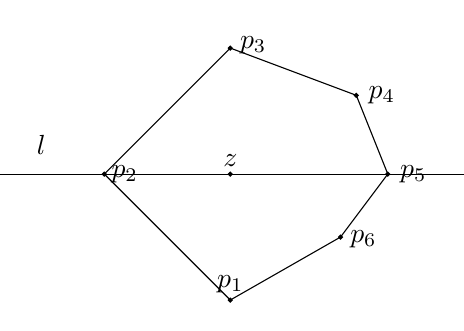
\begin{tikzpicture}[scale=0.8]
      \convex

      \coordinate (z2) at (2,2);
      \coordinate (l2) at (-1,2);

      \draw [shorten >=-3cm, shorten <=-1cm] (l2) -- (z2);

      \node [anchor=center,circle,draw,fill,inner
      sep=0.5pt,label={[anchor=south]below:$z$}] at (z2) {};
      \node [label={[anchor=south]above:$l$}] at (l2) {};
    \end{tikzpicture}
    \caption{Przecięcie zostanie policzone dla krawędzi $p_{2}p_{3}$
      oraz $p_{4}p_{5}$ }
  \end{figure}

\end{itemize}

Ze względu na to, że każdą krawędź $P$ sprawdzamy tylko raz pod względem
przecięcia z $l$, to mamy do czynienia ze złożonością liniową zależną od
liczby krawędzi wielokąta.

Algorytm dla wielokąta wypukłego wymaga pewnego przetwarzania
wstępnego, ale jest użyteczny w przypadku wykonywania wielokrotnych
zapytań o przynależność punktu do danego wielokąta. Weźmy punkt $q$
leżący wewnątrz wielokąta wypukłego $P$, może to być np.\ środek
ciężkości trójkąta wyznaczony przez trzy dowolne jego wierzchołki, a
nastąpnie poprowadźmy $N$ półprostych z $q$ przechodzących przez
wierzchołki $P$. Płaszczyzna wraz z wielokątem zostanie podzielona na
$N$ części, które nazwiemy \emph{klinami}, z których każdy jest podzielony
przez krawędź $P$ na dwie częsci --- jest to wnętrze i zewnętrze
wielokąta.

\begin{figure}[htp]
  \centering
  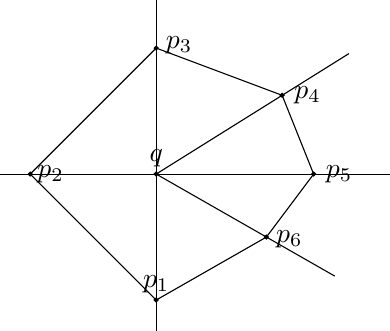
\begin{tikzpicture}[scale=0.8]
    \convex

    \coordinate (z2) at (2,2);

    \draw [shorten >=-1cm] (z2) -- (p1);
    \draw [shorten >=-1cm] (z2) -- (p2);
    \draw [shorten >=-1cm] (z2) -- (p3);
    \draw [shorten >=-1cm] (z2) -- (p4);
    \draw [shorten >=-1cm] (z2) -- (p5);
    \draw [shorten >=-1cm] (z2) -- (p6);

    \node [anchor=center,circle,draw,fill,inner
    sep=0.5pt,label={[anchor=south]below:$q$}] at (z2) {};
  \end{tikzpicture}
  \caption{}
\end{figure}

Wyszukiwanie położenia danego punktu $z$ składa się z dwóch
etapów. Najpierw określany jest klin, w którym leży $z$. Można to
zrobić w czasie $O(\log n)$ używając wyszukiwania binarnego. Punkt $z$
będzie znajdował się pomiędzy promieniami $p_i$ i $p_{i+n}$
podzielonej płaszczyzny wtedy i tylko wtedy, gdy kąt $\angle zqp_i$
będzie lewoskrętny, a kąt $\angle zqp_{i+n}$ prawoskrętny. W
następnych krokach stopniowo zawężamy nasz obszar poszukiwań, do czasu
aż odnajdziemy właściwy klin. Następnie określamy, czy $z$ należy do
wnętrza lub zewnętrza znalezionego klinu. Jeśli kąt $\angle p_{i}p_{i+1}z$
jest lewoskętny to $z$ jest wewnętrzny. Określenie skrętności kąta
jest operacją o czasie $O(1)$, więc asymptotyczna złożoność tej części
algorytmu jest rzędu $O(\log N)$.

Zastosowane tutaj przeszukiwanie binarne jest możliwe dzięki temu, że
wierzchołki wielokąta wypukłego występują w kolejności kątowej lub
inaczej mówiąc w kolejności krążenia wokół punktu $q$. Przetwarzanie
wstępne dla wielokąta $P$ na które składa się wyznaczenie punktu $q$
oraz umieszczenie wielokąta w strukturze danych wspierającej
wyszukiwanie binarne, może zostać wykonane w czasie $O(n)$.

%%% Local Variables:
%%% mode: latex
%%% TeX-master: "masterthesis"
%%% TeX-engine: xetex
%%% End: